\section{Causal analysis}
\label{sec:methods:causal}

\subsection{Potential Outcome Framework}
In order to credibly make the claim that the estimated effect is a causal one, some a priori considerations are in order.
To this end, the review on causal analysis by \citeA{imbens2024causal} is considered.

Firstly, there is the stable unit treatment value assumption (SUTVA), which is the assumption that the outcome for one
individual is not influenced by treatment exposure (in this case, engagement in exercise) of another.
Since the subjects of the LISS panel are selected to be representative of the Netherlands as a whole, the subjects
live all over the country and are not likely to know each other, let alone influence each other. However, it is typical
for multiple individuals to partake within a single household. On average, it is found that about 1.6 individuals participate
per household. Within one household, we cannot rule out that individuals influence each other. In fact, \citeA{maltby2012contextual}
find that one's perception of the benefit of exercise is influenced by social norms, clearly violating the SUTVA.
However, because these violations are local to small groups in the dataset, the assumption is taken to hold at large for
the studied data.

Next, we formalise the effect of interest, namely the causal effect of exercise on mental wellbeing, using the
potential outcome.
For each individual $i$, $Y_i(T)$ is the potential outcome if they engage in exercise (treatment),
and $Y_i(C)$ is the potential outcome if they don't (control). The variable of interest then is the sample average
treatment effect
\begin{equation}
\label{eq:methods:sate}
    \tau_{\text{sample}} = \sum_{i=1}^N (Y_i(T) - Y_i(C)),
\end{equation}
which thanks to the representativeness of the sample is assumed to estimate the population average treatment.
This is where SUTVA is crucial, as without it the potential outcomes are not simply a function of individual $i$'s treatment,
but also of individual $j$'s treatment (where $j \neq i$), and so we could not meaningfully interpret the average
treatment effect calculated as in \cref{eq:methods:sate}.
For any one individual the treatment effect may deviate from the average effect, in the sense that it may be moderated by
for instance personal circumstances or genetics, but such analysis is left to further research.

Denote $X_i$ as the treatment assignment for individual $i$, $X_i \in \{C, T\}$. The crucial assumption is that the
\textit{potential} outcomes are not influenced by the treatment assignment, or formally, given some set of controls
$W_i$,
\begin{equation}
    \label{eq:methods:ignorability_assumption}
    (Y_i(T), Y_i(C)) \perp\!\!\!\perp X_i \mid W_i.
\end{equation}
This assumption is called the ignorability assumption or the assumption of no unobserved confounders.
The controls are included to lend credibility to the assumption, as they remove biases in comparing treated individuals
to individuals in the control group.
Selection bias, MNAR data and the assumption's namesake in no unobserved confounders can all equivalently be considered
violations of the ignorability assumption.
The crucial difficulty that necessitates the assumption is that for any one individual $i$,
only either $Y_i(T)$ or $Y_i(C)$ is observed, and thus we cannot directly observe the difference in potential outcomes.
However, under the ignorability assumption, this difference can be estimated by $Y_i(T) - Y_j(C)$ for $j \neq i$,
which is a quantity that can be observed directly.

Considering the research question at hand is whether physical exercise is an effective intervention, the aim is not to
quantify the exact effect, but rather to find whether a significant effect exists. To that end, the ignorability assumption
can be relaxed slightly to assuming that in so far as there are unmeasured confounders, they do not change the statistical
significance (nor the sign) of the estimated effect.

\subsection{Reverse Causality}
\label{sec:methods:reverse_causality}
Now consider the aim of the present study, namely estimating the effect of exercise on mental health, $Y_i(T) - Y_i(C)$.
In a cross-sectional dataset, this effect is not identified,
because if mental health influences the probability to engage in exercise, the ignorability assumption is violated.
If for instance better mental health makes one more likely to engage in exercise, and assuming the greater mental health
does not disappear as soon as one engages in exercise, then the \textit{potential} outcomes $Y_i$ are increased
for individuals with better mental health. That is, in the observed sample, $Y_i(T) - Y_j(C)$ will be inflated with respect to
$Y_i(T) - Y_i(C)$.
This holds true even if the treatment effect itself is not influenced by a priori mental health.
\Cref{fig:methods:reverse_causality:cs} gives a graphical representation of how the forward and reverse effect
are not simultaneously identified.

On the other hand, with panel data, we can exploit the fact that cause must precede effect. The graphical representation
in \cref{fig:methods:reverse_causality:panel} shows the instantaneous effects, along with presumed
autoregressive effects and a lagged effect.
The latter is now identified. Crucially, the instantaneous effect of sports on MHI5 is not identified, nor is the effect
of lagged sports through the autoregressive behaviour of MHI5.
Recalling that the established mechanisms through which sports may improve mental health can be split into short-term
and long-term mechanisms, it can thus be concluded that observational data provides no way to quantify the short-term effects,
at least not for any effects that last much shorter than the time difference between two waves of the panel.
The elevated endorphin levels post-exercise for instance would likely last on the order of hours (though there is no
research on the exact duration), which is clearly not identifiable on the yearly time-scale of the LISS panel.
Considering the various mechanisms for a positive short-term effect, and assuming a positive long-term effect is found,
it is reasonable to postulate that the short-term effect would also be positive.
Also assuming positive autoregressive coefficients, both the instantaneous effect and the effect through
autoregressive behaviour will also be positive.
To the end of answering the research question then, we may conclude that the total benefit of exercise is at least
as large as the found long-term benefit. Thus, while the unidentified effects mean decreased power in answering
the research question, but significance in the sense of the type I error rate is preserved.
Do note that in a regression context, in order for the effect of SPORTS$_{t-1}$ to be identified with respect to the simultaneous
effects, SPORTS$_t$ should be included as a regressor, as the autoregressive patterns otherwise obscure its effect.

\begin{figure}[htbp]
    \caption{Graph representations of the interactions between MHI5-score and sports. Controls are left out for
    simplicity. Red arrows indicate unidentified effects}
    \label{fig:methods:reverse_causality}
    \begin{subfigure}[t]{0.49\textwidth}
        \centering
        \begin{tikzpicture}[
            node distance=0.8cm,
            main node/.style={circle,draw,font=\scriptsize\sffamily\bfseries,minimum size=1.9cm},
            every edge/.style={draw,thick,->},
        ]
            \node[main node] (mhi5) {MHI5};
            \node[main node, below=of mhi5] (sports) {SPORTS};

            \path[bend left,color=red] (mhi5) edge (sports);
            \path[bend left,color=red] (sports) edge (mhi5);
        \end{tikzpicture}
        \subcaption{Cross-sectional data}
        \label{fig:methods:reverse_causality:cs}
    \end{subfigure}
    \hfill
    \begin{subfigure}[t]{0.49\textwidth}
        \centering
        \begin{tikzpicture}[
            node distance=0.8cm,
            main node/.style={circle,draw,font=\scriptsize\sffamily\bfseries,minimum size=1.9cm},
            every edge/.style={draw,thick,->},
            fading line/.style={draw, thick, dotted, dash pattern=on 2pt off 2pt},
        ]
            \node[main node] (mhi5_t) {MHI5$_t$};
            \node[main node, below=of mhi5_t] (sports_t) {SPORTS$_t$};
            \node[main node, left=1.5cm of mhi5_t] (mhi5_t1) {MHI5$_{t-1}$};
            \node[main node, below=of mhi5_t1] (sports_t1) {SPORTS$_{t-1}$};

            \path[bend left,color=red] (mhi5_t) edge (sports_t);
            \path[bend left,color=red] (sports_t) edge (mhi5_t);
            \path[bend left,color=red] (mhi5_t1) edge (sports_t1);
            \path[bend left,color=red] (sports_t1) edge (mhi5_t1);
            \path (mhi5_t1) edge (mhi5_t);
            \path (sports_t1) edge (sports_t);
            \path[opacity=0.5] (mhi5_t1) edge (sports_t);
            \path[color=green!70!black] (sports_t1) edge (mhi5_t);

            \draw[fading line] ([xshift=-0.6cm]mhi5_t1.west) -- (mhi5_t1.west);
            \draw[fading line] ([xshift=-0.6cm]sports_t1.west) -- (sports_t1.west);
            \draw[fading line] (mhi5_t.east) -- ([xshift=0.6cm]mhi5_t.east);
            \draw[fading line] (sports_t.east) -- ([xshift=0.6cm]sports_t.east);
        \end{tikzpicture}
        \subcaption{Panel data. Note the effect of MHI5$_{t-1}$ on SPORTS$_t$ is identified,
        but is considered a nuisance parameter}
        \label{fig:methods:reverse_causality:panel}
    \end{subfigure}
\end{figure}

While many alternatives exist, for the present research, the package \textit{lavaan} in R is used \cite{rosseel2012lavaan}.
This choice was made because \textit{lavaan} is a mature and feature-rich project, whose reliability is exemplified by its
extensive use in the literature.

\section{Structural Equation Modelling}
\label{sec:methods:sem}
SEM can be considered a generalisation of the linear model, where rather than one regression equation which explains
the variability of the regressand with regards to a set of regressors, multiple regression equations are estimated simultaneously
to explain the total covariance structure of all variables involved.
The following will be a minimal introduction for the purpose of this work, in which accuracy is sacrificed to some degree
in favour of simplicity.
For a full introduction, consider textbooks such as \citeA{kline2023principles}.
While SEM also allows for modelling latent variables in its general form, such constructs are not considered
in this work. This is because the author possesses no a priori knowledge as to what latent constructs might exist, and
\citeA{ludtke2022comparison} find in a simulation study that empirically deciding on latent structures ``is only
of limited usefulness, because the different model[l]ing approaches provide almost equivalent representations of [the data].''

Consider then a vector $z_i$, which contains for individual $i$ the outcome variable of interest $y_i$ as well as
all regressors $x$.
For the purpose of maximum likelihood estimation of the population parameters, note the well-known
likelihood (density) of a single observation
\begin{equation}
    f(z_i; \mu, \Sigma) = (2\pi)^{-\frac{p}{2}} |\Sigma|^{-\frac{1}{2}} e^{-\frac{1}{2}(z_i - \mu)' \Sigma^{-1}(z_i - \mu)},
\end{equation}
where $p$ denotes the dimension of $z_i$.
Assuming independent observations and dropping the constant, the sample log likelihood is
\begin{equation}
    \label{eq:methods:sample_likelihood}
    l(z) = \sum_{i=1}^N \log(f(z_i; \mu, \Sigma))
    = -\frac{N}{2} \log(|\Sigma|) -\frac{1}{2} \sum_{i=1}^N (z_i - \mu)' \Sigma^{-1} (z_i - \mu),
\end{equation}
which for the purposes of optimisation can be rewritten to an equivalent fit function $F$, defined in terms of
the sample mean $\bar{x}$ and covariance matrix $S$ \cite{preacher2016ml} as
\begin{equation}
    \label{eq:methods:objective_function}
    F(\mu, \Sigma) = \log|\Sigma| + \text{tr}(S \Sigma^{-1}) - \log|S| - p + (\bar{z} - \mu)' \Sigma^{-1} (\bar{x} - \mu),
\end{equation}
with tr($\cdot$) denoting the trace of a matrix and the minimum of $F$ coincides with the maximum likelihood estimate.
Note this fit function does not directly involve any observation $z_i$. Rather it is defined purely in terms of the
sample moments $\bar{z}$ and $S$, which is to say that while \cref{eq:methods:sample_likelihood} and
\cref{eq:methods:objective_function} are theoretically equivalent, the latter operates on a higher level of abstraction.

At this stage, the elements of $\mu$ and $\Sigma$ may be estimated directly through numerical optimisation.
Firstly, note that $\mu$ can always be estimated as $\hat{\mu} = \bar{z}$, such that the last term in
\cref{eq:methods:objective_function} vanishes. It can thus be estimated separately from $\Sigma$,
and because the research question pertains specifically to the variability of variables,
the mean term is ignored in further discussion.
To see how this general multivariate likelihood approach relates to the linear model, consider the very simple example
regression of
\begin{equation}
    \label{eq:methods:simple_regression}
    y = \alpha + \beta_1 x_1 + \beta_2 x_2 + \epsilon.
\end{equation}
From this equation, the model-implied covariances between $y$
and $x_1$ and $x_2$ can be readily defined in terms of the regressor covariances as
\begin{align}
\begin{split}
    \label{eq:methods:covariance_simple_regression}
    \Sigma_{y x_1} &= \beta_1 \Sigma_{x_1} + \beta_2 \Sigma_{x_1 x_2}\text{ and} \\
    \Sigma_{y x_2} &= \beta_1 \Sigma_{x_1 x_2} + \beta_2 \Sigma_{x_2},
\end{split}
\end{align}
where $\Sigma_{x_1}$ ($\Sigma_{x_2}$) denotes the variance of $x_1$ ($x_2$) and $\Sigma_{x_1 x_2}$ denotes the covariance between $x_1$ and $x_2$.
Estimating $\Sigma_{y x_1}$ and $\Sigma_{y x_2}$ thus corresponds directly to estimating $\beta_1$ and $\beta_2$.
In general, the upper-right row of elements of the covariance matrix of $z$ is $\Sigma_{xy} = \Sigma_x \beta$ for
a vector of regressors $x$ and a vector of parameters $\beta$, where $\Sigma_x$ is the covariance matrix of $x$.
For completeness, the diagonal elements of $\Sigma$ are estimated directly as well as the covariance elements between
the regressors, at which point estimating the above regression equation is just a matter of reparametrisation as compared
to estimating the corresponding elements of $\Sigma$ directly; the two approaches are completely equivalent.

A benefit of the higher-level abstraction in SEM as compared the canonical linear model, is that multiple regressions
can be estimated simultaneously. Consider for instance
\begin{align}
\begin{split}
    \label{eq:methods:simultaneous_regression}
    y_1 &= \alpha_1 + \gamma y_2 + \epsilon_1;\\
    y_2 &= \alpha_2 + \beta x + \epsilon_2.
\end{split}
\end{align}
Note the subscripts in $y_1$ and $y_2$ denote different variables altogether,
not necessarily the same variable at different points in time.
Now, the model-implied $\Sigma_{y_1 x} = \gamma \beta \Sigma_x$.
However, because in general the second equation in \cref{eq:methods:simultaneous_regression} does not fully explain the
variance in $y_2$ ($R^2 < 1$), this may not fully explain the covariance between $y_1$ and $x$.
That is, there may be a residual covariance $\phi_{y_1 x}$, such that $\Sigma_{y_1 x} = \gamma \beta \Sigma_x + \phi_{y_1 x}$.
Note also that with three total variables, there are three covariance elements in $\Sigma$, but $\{\gamma, \beta\}$
constitutes only two parameters to estimate, which is too few parameters to exactly estimate the full covariance structure.
Additionally, $\Sigma_{y_1} = \phi_{y_1} + \gamma \phi_{y_2} + \gamma \beta \Sigma_x$, where
$\phi_{y_1}$ denotes the residual variance of $y_1$ and likewise $\phi_{y_2}$. That is, the variance of $y_1$ is not
just defined in terms of its regressors, but also in terms of its regressors' regressors (and so on).

A general implication of the higher level of abstraction is that while canonically, the linear model has $N - k$ degrees
of freedom if there are $k$ parameters to be estimated, in SEM there are $\frac{p(p+1)}{2} - k$ degrees of freedom
for a model that involves $p$ variables. Note $\frac{p(p+1)}{2}$ is the number of unique elements in the covariance matrix.
For example, the model in \cref{eq:methods:simple_regression} involves three variables (again, neglecting the mean component),
so again three covariance elements in $\Sigma$. Two of these are implied as in \cref{eq:methods:covariance_simple_regression},
but because both $x_1$ and $x_2$ only show up as regressors, the model does not imply any structure to their covariance,
and it is simply estimated as $\Sigma_{x_1 x_2} = \phi_{x_1 x_2}$. The residual variance of $y$ is also estimated along
with the two variances of the regressors, which leaves $\frac{p(p + 1)}{2} - k = 6 - 6 = 0$ degrees of freedom. This is
referred to as a model that is just identified.
The model in \cref{eq:methods:simultaneous_regression} differs in that it implies all three covariances, but with only two
parameters. If the model is not supplemented with $\phi_{y_1 x}$, there is $6 - 5 = 1$ degree of freedom, which is to
say that the model is overidentified.
While the example is trivial, in a more complex model we may exploit overidentification to quantify
whether the proposed model adequately describes the data. In other words, fit indices can be derived from these degrees
of freedom, in some sense analogous to the Sargan-Hansen test for the generalised method of moments.

A model specification in SEM is simply the set of regression pathways and residual variances to be estimated as free
parameters.
SEM lends itself well to the present research, because it necessitates very few restrictions on the model.
This makes it a natural choice for exploring a potentially complex and unknown relationship between variables.
A panel regression fits into the SEM framework by having one regression for each wave of the panel,
i.e. $y_{i,1} = \ldots; y_{i, 2} = \ldots$, and so on. The framework then allows for instance adding autoregressive terms
(dynamic panels), having (co)variances vary across waves or even two-way fixed effects
(i.e. time dummies and individual-specific effects).
Fundamentally, the only restriction imposed by SEM is that the covariance matrix is sufficient to identify the parameters.
Notably, while Arellano-Bond (AB) estimation of dynamic panel models relies on first-differencing the model for identification,
SEM does not and as such it is possible to include time-invariant controls beyond just the catch-all individual-specific effect.
Additionally, AB estimation necessitates on a choice of instruments which compromise model validity if inappropriate
\cite{bazzi2013blunt}, and SEM was empirically found to be more efficient than AB \cite{leszczensky2022deal}.
Altogether, SEM is the preferred choice for the present study.

\subsection{Fixed and Free Parameters}
\label{sec:methods:fixed_free_parameters}
In \textit{lavaan}, a parameter can either be fixed to a specific value or estimated freely.
There are two forms of parameters, namely regression coefficients and additional (residual) covariances (i.e. $\phi_{x_1 x_2}$).
If a variable is a regressand or if one of its covariances is set as a free parameter, then all of its covariances
must be either estimated through free parameters or fixed to zero to ensure the model-implied covariance matrix is
positive definite.
In that sense, it is meaningful to talk about a variable as whole to be treated as fixed or not.

Treating variables as fixed makes it impossible to examine the covariances between them,
for instance to test whether $\text{Cov}(x_1, x_2) = 0$.
However, for the present work, the choice to treat all regressors as fixed comes naturally,
because the covariance structure between regressors is not relevant to the research question;
doing so improves model parsimony;
and considering fit indices are defined in terms of the degrees of freedom,
a good model fit in terms of the regressors may obscure a poor model fit for the outcome variable,
decreasing the indices' value to the present study.

\subsection{Panel Model Formulation}
\label{sec:methods:model_formulation}
The following model formulation is adapted from \citeA{allison2017maximum}.
In a simplified form, the central regression equation is
\begin{equation}
    \label{eq:methods:model_formulation}
    y_{it} = \alpha_t + \alpha_i + \rho y_{i,t-1} + \beta x_{it} + \omega' w_{it} + \delta' z_i + \epsilon_{it}.
\end{equation}
$y_{it}$ is the MHI5-score of individual $i$ at time $t$ while $\alpha_t$ represents a time dummy,
$x_{it}$ exercise status, $w_{it}$ is a vector of time-varying controls and $z_i$ a vector of time-invariant controls.
This equation is simplified in the sense that it only contains a single autoregressive (AR) term and a single lag of $x$,
i.e. no distributed lags (DL). This is not a necessary restriction, but is done here for simplicity.
The selection of lags for the final model is discussed in \cref{sec:modelling:lags}. The model has to be complemented
with the initial conditions for $y$. If only one autoregressive lag is included, only $y_{i,1}$ is required,
but for a higher lag order more initial conditions are required. If distributed lags are included, then likewise for $x$.
A practical implication of this is that the higher the autoregressive (distributed) lag order, the fewer waves
are available for analysis. This is especially relevant in the present study, because the missingness of the MHI5-score
in 2014 means twice as many waves are lost as would be the case if the Health study had been conducted that year.
The fact that time-invariant controls $z_i$ may be included is beneficial for controls that vary so little in time that
treating subsequent values as separate variables causes numerical instability (colinearity). For such a variable,
the first observed (non-NA) value of each individual is used as the time-invariant approximation. While this choice
is ambiguous, the very fact that the variable must be modelled as a time-invariant implies that the exact
choice of approximation matters very little.

The main identifying assumption is \cite{moral2019dynamic}
\begin{equation}
    \label{eq:methods:identifying_assumption}
    E(\epsilon_{it} | y_i^{t-1}, x_i^t, \alpha_t, w_{i}^t, z_i) = 0 \,\forall\,\{i,t\},
\end{equation}
where a superscript $t$ denotes all observations of the corresponding variable up to time $t$.
Verbally, the assumption entails that all included regressors are exogenous.
Note the exogeneity of $x$ is also implied by the ignorability assumption (\cref{eq:methods:ignorability_assumption}).
Furthermore, while all regressors are included in the identifying assumption, if a control is endogenous it simply
leads to inconsistent estimation of the corresponding parameter, that has a weaker influence on the estimation
of the parameter of interest ($\beta$) than endogeneity of $x$ itself, and is thus of lesser concern in practice.
Beyond \cref{eq:methods:identifying_assumption}, in a random effects specification, the time-invariant controls
must also be uncorrelated with the individual-specific effects, in order to differentiate between $\alpha_i$ and $\delta$.

The effect $\beta$ in \cref{eq:methods:model_formulation} cannot be interpreted directly as the effect that $x$ (exercise)
has at time $t$ on $y$ (MHI5-score), due to the autoregressive behaviour. However, it can be interpreted as a change
in the equilibrium value of $y_{it}$. Namely, if for an individual $x_{it}$ changes from 0 to 1, i.e. they did not
engage in exercise but have started doing so, they equilibrium value of $y_{it}$ changes by
\begin{equation}
    \label{eq:methods:long_run_effect}
    \frac{\sum_{l=0}^{L_x} \beta_l}{1 - \sum_{l=1}^{L_y} \rho_l}
\end{equation}
where $L_x$ denotes the distributed lag order and $L_y$ denotes the autoregressive lag order.
Refer to \cref{chap:app:long_run_effect} for a derivation.

To briefly note, \cref{eq:methods:model_formulation} assumes a linear influence of all regressors onto $y$. However, all regressors
are included as dummies, i.e. on a binary scale. For such a scale, linearity holds exactly.
The only exception is the autoregressive terms, but since even a small number of autoregressive terms can already
model highly nonlinear temporal behaviour, it is likely a reasonable approximation.

\subsection{Controls and Mediators}
\label{sec:methods:controls_mediators}
As discussed extensively already, the selection of controls is crucial to avoid unmeasured confounders. However,
a second important consideration is the action of mediators. Mediators are variables that explain the effect
of $x$ on $y$, in the sense that $x$ causes some mediator $m$ which causes $y$. An example of a mediator in the present
study might be physical health. If physical health is included as a control in the regression, the interpretation of $\beta$
becomes ``the effect of sports on MHI5-score, \textit{given} the physical health status of an individual.'' However,
improvement of physical health may well be a strong mechanism through which sports affects mental health, which
should very much be included in $\beta$ for the purpose of answering the research question. The subtleties of mediation
are often not discussed in the literature \cite{imbens2024causal}, e.g. \citeA{chekroud2018association} simply include physical health as a control.
Such mediation might be measured directly while still effectively controlling for confoundedness due to the mediator as
in the following, simplified example:
\begin{align}
\begin{split}
    \label{eq:methods:mediation_example}
    y_{it} &= \alpha_y + \beta x_{it} + \eta m_{it} + \epsilon_y; \\
    m_{it} &= \alpha_m + \zeta x_{it} + \epsilon_m.
\end{split}
\end{align}
Then, the total effect of $x$ on $y$ is given as $\beta + \zeta \eta$, the sum of the direct and the indirect effects.
Conveniently, these two regressions may be estimated simultaneously in SEM.

Thus, when determining the controls used, attention must be paid to which variables may be mediators and those should be
modelled as in \cref{eq:methods:mediation_example}. There is a significant price to be paid in terms of model parsimony
though, as a mediator cannot be a fixed variable, potentially adding many additional parameters to the model.
If a mediator is simply excluded from the regression altogether, this model complexity is avoided, while the indirect
effect (e.g. $\zeta \eta$) is absorbed into the main parameter ($\beta$). However, in doing so, the mediator, in so far
as it is not fully explained by $x$, also functions as a potential unmeasured confounder.
Because it is not clear a priori which approach is preferred, the results for both will be given in the present study.
In this way, it can also be directly examined to which degree the mediators are confounders by comparing
the estimated coefficients $\beta$ between the two approaches.

When multiple mediators are simultaneously modelled, there can be either parallel mediation or serial mediation \cite{hayes2017introduction}.
In parallel mediation (\cref{fig:methods:mediation_forms:parallel}), the mediators do not influence each other,
whereas in serial mediation (\cref{fig:methods:mediation_forms:serial}) one mediator causes the next mediator.
If multiple mediators affect each other and the outcome variable as in \cref{fig:methods:mediation_forms:simultaneous},
there is another form of simultaneity in the model. While this could be modelled with panel data just as the main
simultaneity is modelled in the present study, that would entail significant model complexity.
Instead, the present study models multiple mediators as parallel mediation, which effectively makes the assumption that,
conditional on the set of controls and sports, there is no causal dependence between the mediators.
The residual covariance of the mediators can be estimated in the SEM model to what extent this approximation holds.
Clearly, different dummy levels of the same categorical mediator must be causally dependent, which necessarily
compromises the findings.

\begin{figure}[htbp]
    \caption{Graph representations of different forms of mediation}
    \label{fig:methods:mediation_forms}
    \begin{subfigure}[t]{0.32\textwidth}
        \centering
        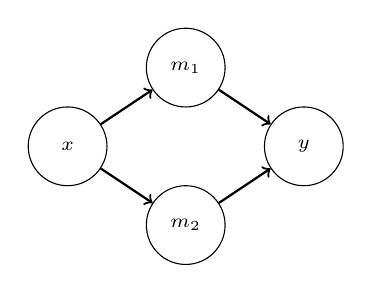
\begin{tikzpicture}[
            node distance=0.4cm,
            main node/.style={circle,draw,font=\scriptsize\sffamily\bfseries,minimum size=1cm},
            every edge/.style={draw,thick,->},
        ]
            \node[main node] (m1) at (0, 2) {$m_1$};
            \node[main node] (m2) at (0, 0) {$m_2$};
            \node[main node] (x) at (-1.5, 1) {$x$};
            \node[main node] (y) at (1.5, 1) {$y$};

            \path (x) edge (m1);
            \path (x) edge (m2);
            \path (m1) edge (y);
            \path (m2) edge (y);
        \end{tikzpicture}
        \subcaption{Parallel mediation}
        \label{fig:methods:mediation_forms:parallel}
    \end{subfigure}
    \hfill
    \begin{subfigure}[t]{0.32\textwidth}
        \centering
        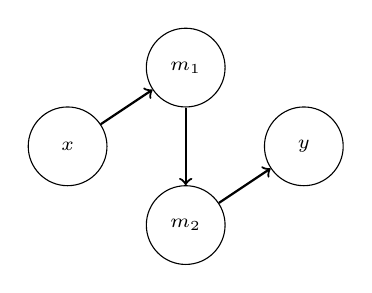
\begin{tikzpicture}[
            node distance=0.4cm,
            main node/.style={circle,draw,font=\scriptsize\sffamily\bfseries,minimum size=1cm},
            every edge/.style={draw,thick,->},
            fading line/.style={draw, thick, dotted, dash pattern=on 2pt off 2pt},
        ]
            \node[main node] (m1) at (0, 2) {$m_1$};
            \node[main node] (m2) at (0, 0) {$m_2$};
            \node[main node] (x) at (-1.5, 1) {$x$};
            \node[main node] (y) at (1.5, 1) {$y$};

            \path (x) edge (m1);
            \path (m2) edge (y);
            \path (m1) edge (m2);
        \end{tikzpicture}
        \subcaption{Serial mediation}
        \label{fig:methods:mediation_forms:serial}
    \end{subfigure}
    \hfill
    \begin{subfigure}[t]{0.32\textwidth}
        \centering
        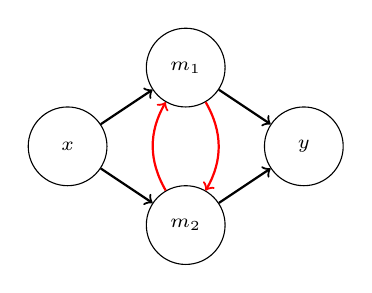
\begin{tikzpicture}[
            node distance=0.4cm,
            main node/.style={circle,draw,font=\scriptsize\sffamily\bfseries,minimum size=1cm},
            every edge/.style={draw,thick,->},
            fading line/.style={draw, thick, dotted, dash pattern=on 2pt off 2pt},
        ]
            \node[main node] (m1) at (0, 2) {$m_1$};
            \node[main node] (m2) at (0, 0) {$m_2$};
            \node[main node] (x) at (-1.5, 1) {$x$};
            \node[main node] (y) at (1.5, 1) {$y$};

            \path (x) edge (m1);
            \path (x) edge (m2);
            \path (m1) edge (y);
            \path (m2) edge (y);
            \path[bend left,color=red] (m1) edge (m2);
            \path[bend left,color=red] (m2) edge (m1);
        \end{tikzpicture}
        \subcaption{Simultaneity in mediation}
        \label{fig:methods:mediation_forms:simultaneous}
    \end{subfigure}
\end{figure}

The simplified example in \cref{eq:methods:mediation_example} does not include controls or autoregression. In order for the parameters $\zeta$ and $\eta$
to be meaningfully combined, the same set of controls should be present in the mediation regression as in the main
regression. Because of this, all the regressors in the main regression are added to the mediation regression, including
the lagged $y_{i,t-l}$. However, because of the modelling choice of parallel mediation, mediators are not included
in the mediation regressions of other mediators.

An additional concern in mediation is that the mediator may also be a vehicle for the reverse effect.
Just as $\beta$ in \cref{eq:methods:mediation_example} cannot differentiate between the forward- and reverse effects,
neither can $\eta$ nor $\zeta$. That is, in mediation, there is a concern for both the reverse effect of $y_{it}$ onto
$m_{it}$ and the reverse effect of $m_{it}$ onto $x_{it}$. Just as in \cref{fig:methods:reverse_causality:panel},
we may measure only lagged effects in both equations, at the cost of model parsimony and only being able to judge the
effect of $x_{i,t-2}$ on $y_{it}$.
If on mechanistic grounds the reverse causality in either equation is expected to be negligible, it can be justified
to measure the instantaneous effect in that regression.
For the interpretation of the long-run effect of $x$, \cref{eq:methods:long_run_effect} shows that each lag $\beta_l$
has the same influence on the outcome. As such, regardless of the lag structure decided on in mediation, the sum of the
direct and indirect effects can be meaningfully interpreted as the total effect.

Because mediators cannot be treated as fixed variables, a consideration is which of their residual covariances
to set as free parameters.
While there may be autoregressive behaviour for the mediator variables, this is controlled for by
setting the covariance between any two consecutive values of mediators as a free parameter, with these parameters
being allowed to vary freely across time to eliminate all associated degrees of freedom.
An implication of this is that if in reality there is AR behaviour to the mediators, the total
effect of sports through them is underestimated (assuming positive AR coefficients).
The approximation thus maintains type I significance.
The AR nature could also be explicitly modelled, but doing so would make modelling much more complex and error-prone,
so the fact that $\alpha$-significance is maintained justifies accepting the reduced statistical power as a compromise.
Additionally, if a mediator is a categorical variable, there must be a negative correlation between its different
dummy variables, so correlations between different dummy levels of the same variable are also set as free parameters.

\subsection{Fit Indices}
\label{sec:methods:fit_indices}
There is an extensive set of fit indices for SEM models available in the literature. These derive from the degrees of freedom
in various ways. No single fit index is definitive for model fit, so it is prudent to consider multiple together
for a more complete view. A canonical set of fit indices is described hereafter. However, two general remarks are in order.
Firstly, if a model is just identified, each of these fit indices will always indicate a perfect fit, which is to
say there is then no value in interpreting the indices.
Secondly, these tests do not necessarily provide a way to compare competing models. Considering they all measure the
extent to which the model-implied covariance matrix differs from the sample covariance matrix, if two competing models
involve a different set of variables, the indices cannot be directly compared. That is, if model A fits the sample
covariance matrix $S_A$ better than model B fits $S_B$, it does not necessarily follow that model A is better than model B.
For example, a model which has no controls would likely yield better fit indices because it is a much simpler model
with fewer parameters to be estimated,
but that does not make it the preferred model over a model which includes a set of relevant control variables.
\Cref{sec:methods:cv} will discuss the alternative approach used in this work for model selection.

\subsubsection{$\chi^2$ test}
The $\chi^2$ test is the most general (and the original) fit index used \cite{smith2001primer}. It is a badness-of-fit
test, in the sense that the null hypothesis is that the model explains the data perfectly. To be precise,
the test statistic is the discrepancy between the model-implied covariance matrix, and a significant test result
thus implies the null is rejected, implying a significant discrepancy.
In practice with ML estimation, the test statistic is calculated as
\begin{equation}
    \label{eq:methods:chi2_test_stat}
    \chi^2 = (N - 1) F(\hat{\Sigma}),
\end{equation}
where $F(\cdot)$ is the objective function as in \cref{eq:methods:objective_function}.
Under the null, the statistic is distributed as $\chi^2_{df}$ if the model has $df = \frac{p(p + 1)}{2} - k$ degrees of freedom
\cite{zheng2025enhancing}.

However, a shortcoming of the $\chi^2$ test is that it is sensitive to sample size, in the sense that as
the number of observations $N$ increases, the null is less likely to be maintained. This is not a
desirable property of a fit index, which has given rise to other fit indices \cite{smith2001primer}.
As an alternative, \citeA{joreskog1993lisrel} propose using the ratio $\chi^2 / df$ as an indicator of goodness-of-fit,
where a ratio below 2 represents ``good'' fit and below 3 ``acceptable''. However, this does not fundamentally eliminate
the sensitivity to sample size; rather, it just proposes more lenient critical values.

\subsubsection{Comparative Fit Index (CFI)}
The CFI derives from the $\chi^2$ test. It compares the $\chi^2$ test statistic of the model to that of a baseline model.
While what constitutes the baseline model is subjective (f.i. \citeA{van2021understanding}), typically the baseline model is a
model in which the variances of all variables are estimated, whereas the covariances are not (i.e. fixed to 0).
The statistic is then
\begin{equation}
    \text{CFI} = 1 - \frac{\max(\chi^2 - df, 0)}{\max(\chi^2 - df, \chi^2_b - df_b, 0)}.
\end{equation}
Here, $\chi^2$ and $df$ denote the test statistic and degrees of freedom of the model and the same variables with a
subscript $b$ are those of the baseline model \cite{schermelleh2003evaluating}.
While no analytical distribution is available for this statistic, its value is in the range $[0, 1]$, with a
higher value indicating better fit. It reaches a value of 1 if the ratio of $\chi^2$ to $df$ is less than 1,
and a value of 0 if the baseline model fits the data better than the proposed model.
Typically a cutoff value of $0.95$ is taken to indicate good model fit \cite{hu1999cutoff}.

\subsubsection{Tucket-Lews Index (TLI)}
Similar to the CFI, \citeA{schermelleh2003evaluating} define the TLI as
\begin{equation}
    \text{TLI} = \frac{\chi_b^2 / df_b - \chi^2 / df}{\chi_b^2 / df_b - 1}.
\end{equation}
While not strictly confined to the range of $[0, 1]$, the TLI is typically in that range, only exceeding it
if the baseline model outperforms the proposed model, or if model fit is so good as to make $\chi^2 < df$.
Again, higher is better, and the cutoff for good fit is taken from \citeA{hu1999cutoff} as 0.95.

\subsubsection{Root Mean Square Error of Approximation (RMSEA)}
The RMSEA measures the discrepancy between the model-implied- and sample covariance matrices per degree of freedom,
roughly defined as the root mean square difference between the two \cite{schermelleh2003evaluating}.
It improves on the $\chi^2$ statistic by compensating for the degrees of freedom and the sample size.
\begin{equation}
    \text{RMSEA}^2 = \frac{\max(\chi^2 - df, 0)}{df(N - 1)}.
\end{equation}
The RMSEA has a lower bound of 0 and no upper bound, with a lower RMSEA representing better fit.
We use a cutoff of 0.06 to indicate good fit \cite{hu1999cutoff}.

\subsubsection{Standardised Root Mean Square Residual (SRMR)}
Lastly, the SRMR is defined most explicitly in terms of $S - \hat{\Sigma}$ without considering degrees of freedom,
namely as \cite{schermelleh2003evaluating}
\begin{equation}
    \text{SRMR}^2 = \frac{\sum_{i=1}^p\sum_{j=1}^i (\frac{S_{ij} - \hat{\Sigma}_{ij}}{S_i S_j})^2}{p(p+1)/2}.
\end{equation}
The term being summed is the (square) discrepancy between $S$ and $\hat{\Sigma}$, standardised with respect to the sample standard
deviations $S_i$ and $S_j$ to eliminate dependence on the scale of variables.
Again, it has no upper bound but is bounded below by 0, and lower values indicate better fit.
The cutoff used is 0.08 \cite{hu1999cutoff}.

\subsection{Cross Validation}
\label{sec:methods:cv}
For the sake of model selection, a model-agnostic measure of model fit is required. To this end, we may borrow from the
machine learning literature and use out-of-sample forecasting accuracy through cross validation.
This approach can be used to compare any two models, including non-nested ones, and is a fit measure more akin to those
used in canonical linear modelling.
However, as mentioned before, when comparing different autoregressive lag orders, the lower lag order will have
more waves available. It is likely that a model fit to a larger number of waves has a worse fit due to slight
unmodelled heterogeneity across the waves, making the comparison between models unfair. Because of this, only the last
available wave (2023) is used for cross validation, both for fitting the models as well as for determining the forecasting
accuracy. It does not necessarily hold that the model that best fits the final wave is the one that best fits
the data as whole, but it is nevertheless taken as a necessary and reasonable approximation.

In model selection, accuracy must be balanced with parsimony. To this end, the decision rule used is the 1-$\sigma$ rule,
where the model chosen is the simplest model whose out-of-sample forecasting accuracy is within one standard deviation
of the best-performing model. Specifically, across the $v$ folds, the root mean square prediction error (RMSPE)
$\mu_{\text{RMSPE}}$ is calculated, along with the standard deviation of this prediction error across the folds,
$\sigma_{\text{RMSPE}}$. The simplest model whose $\mu_{\text{RMSPE}}$ is below the optimal model's
$\mu_{\text{RMSPE},opt} + \sigma_{\text{RMSPE},opt}$ is selected.
In this, the number of folds $v$ plays a critical role, as when more folds are used, the training sets are larger
and the testing sets are smaller, which generally leads to lower $\mu_{\text{RMSPE}}$. Typical values are $v = 5$ or
$v = 10$. The dataset at hand is large, but considering the high percentage of missing data, a smaller number for
$v$ is preferred to avoid unrepresentative test sets, so $v = 5$ is used.
To improve the accuracy of the estimated $\mu_{\text{RMSPE}}$ and $\sigma_{\text{RMSPE}}$, this cross validation
is repeated $R$ times with different random folds in each repetition and the average estimates is taken.
Here, the larger $R$ the better, but $R = 50$ is chosen to balance precision and computational tractability.
Because uncertainty in the estimates has a significant impact on the 1-$\sigma$ decision rule,
the uncertainties in the estimates of $\mu_{\text{RMSPE}}$ and $\sigma_{\text{RMSPE}}$ are calculated as the standard
deviation of the respective estimates across the repetitions divided by the square root of $R$.
The uncertainty of the decision rule threshold is then found by quadratically adding these two uncertainties.
There is the possibility that the model used is not identified or numerically unstable for a given split due to the high
degree of missingness. When this occurs, the results for the current repetition are discarded and another repetition is
done.

\subsection{Full Information Maximum Likelihood}
\label{sec:methods:fiml}
SEM, at least when combined with maximum likelihood estimation, provides a natural way to handle (MAR) missing data in the
form of Full Information Maximum Likelihood (FIML) \cite{arbuckle2013full}.
The basic premise of FIML is that if a variable is missing for some observation, that observation provides no information
as to how the missing variable relates to other variables, but it still provides information for the remaining variables.
Formally, consider estimation of the covariance matrix $\Sigma$ of the vector $x' = (x_1, x_2, x_3)$.
Because the total sample likelihood (\cref{eq:methods:sample_likelihood}) is the product of the likelihood of each observation,
we need not necessarily use the same likelihood specification for each observation.
If for some observations $x_3$ is missing, their contribution to the likelihood is simply calculated with the two-dimensional
covariance matrix of the sub-vector $(x_1, x_2)'$.
In this way, FIML uses all information available in the dataset, hence its name. It can be applied to regressors
as well as to regressands, making it highly valuable for the present study.
It is not, however, a solution to a variable completely missing from the data, as is for instance the case with the
missing Health study in 2014. In that case there is no information in the sample altogether, i.e. the sample covariance
is not known and thus cannot be fit to.

\textit{Lavaan} provides the option to apply FIML only to the endogenous variables or to all variables.
If FIML is only applied to the endogenous variables, listwise deletion is applied for those cases where the exogenous
variables are missing. As doing so would eliminate a large portion of the data, FIML is used for all variables in the dataset.

\subsection{Normality and Robust Maximum Likelihood}
\label{sec:methods:normality_mlr}
The derivation of the objective function in \cref{eq:methods:objective_function} relies heavily on the assumption
of normality. However, while this assumption might hold approximately for the MHI5-score, it clearly does not hold
for all the binary regressors. This is of no concern for exogenous variables, as their covariances are simply fixed
to the sample covariance, but it does implicate the parameter of interest, namely the effect of exercise on MHI5.
Even so, \citeA{knief2021violating} find that the normal estimator still behaves well in terms of bias and
efficiency. They even argue that it may be preferable to violate the assumption of normality over using specific
techniques to adjust for non-normality, as those are error prone.
Nevertheless, it would seem worthwhile to use robust approach to maximum likelihood estimation that are readily
available in \textit{lavaan}. While multiple choices exist, ML with Huber-White standard errors is used (often
referred to as ``MLR''), as it was found to perform well in the face of nonnormality \cite{zhong2011bias}, while
still allowing for the use of FIML which some robust alternatives prohibit.
With MLR in \textit{lavaan}, a robust alternative to the $\chi^2$ statistic is also calculated as in \citeA{satorra2001scaled},
which means it and the fit indices that derive from it are also robust.
In practice it was found that bootstrap standard errors align well with the standard errors implied by MLR estimation,
whereas SEs with regular maximum likelihood were appreciably smaller, which corroborates the decision to prefer
robust estimation.
